\documentclass{beamer}
\usepackage[utf8]{inputenc}
\usepackage[T1]{fontenc}
\usepackage{graphicx}
\usepackage{booktabs}
\usepackage{hyperref}

% --- Theme Configuration ---
\usetheme{Madrid}
\usecolortheme{default}

% --- Title Page ---
\title[Análise de Performance Educacional]{Análise da Influência do Espectro Político na Performance Educacional dos Municípios}
\author{Seu Nome}
\institute{Universidade Federal do Ceará \\ Disciplina: Engenharia de Sistemas Inteligentes (CK0444)}
\date{\today}

\begin{document}

% --- Slide 1: Title ---
\begin{frame}
    \titlepage
\end{frame}

% --- Slide 2: Project Architecture ---
\begin{frame}{Arquitetura do Projeto: Pipeline MLOps}
    \begin{itemize}
        \item<1-> \textbf{Pipeline de Dados (`sdp-data`):} Coleta, limpa e combina dados do INEP e TSE.
        \item<2-> \textbf{Pipeline de Modelo (`sdp-model`):} Treina, avalia e seleciona um modelo de classificação (RandomForest).
        \item<3-> \textbf{Serviço de API (`sdp-service`):} Expõe o modelo treinado via API REST para predições em tempo real.
        \item<4-> \textbf{Automação (GitHub Actions):} Orquestra todo o fluxo de CI/CD, garantindo a integridade e reprodutibilidade do projeto.
    \end{itemize}
    \vfill
    \begin{center}
    \includegraphics<5->[width=0.9\textwidth]{assets/desempenho_espectro.png}
    \end{center}
\end{frame}

% --- Slide 3: Exploratory Data Analysis ---
\begin{frame}{Análise Exploratória dos Dados}
    \begin{columns}[T]
        \begin{column}{0.5\textwidth}
            \textbf{Desempenho por Espectro}
            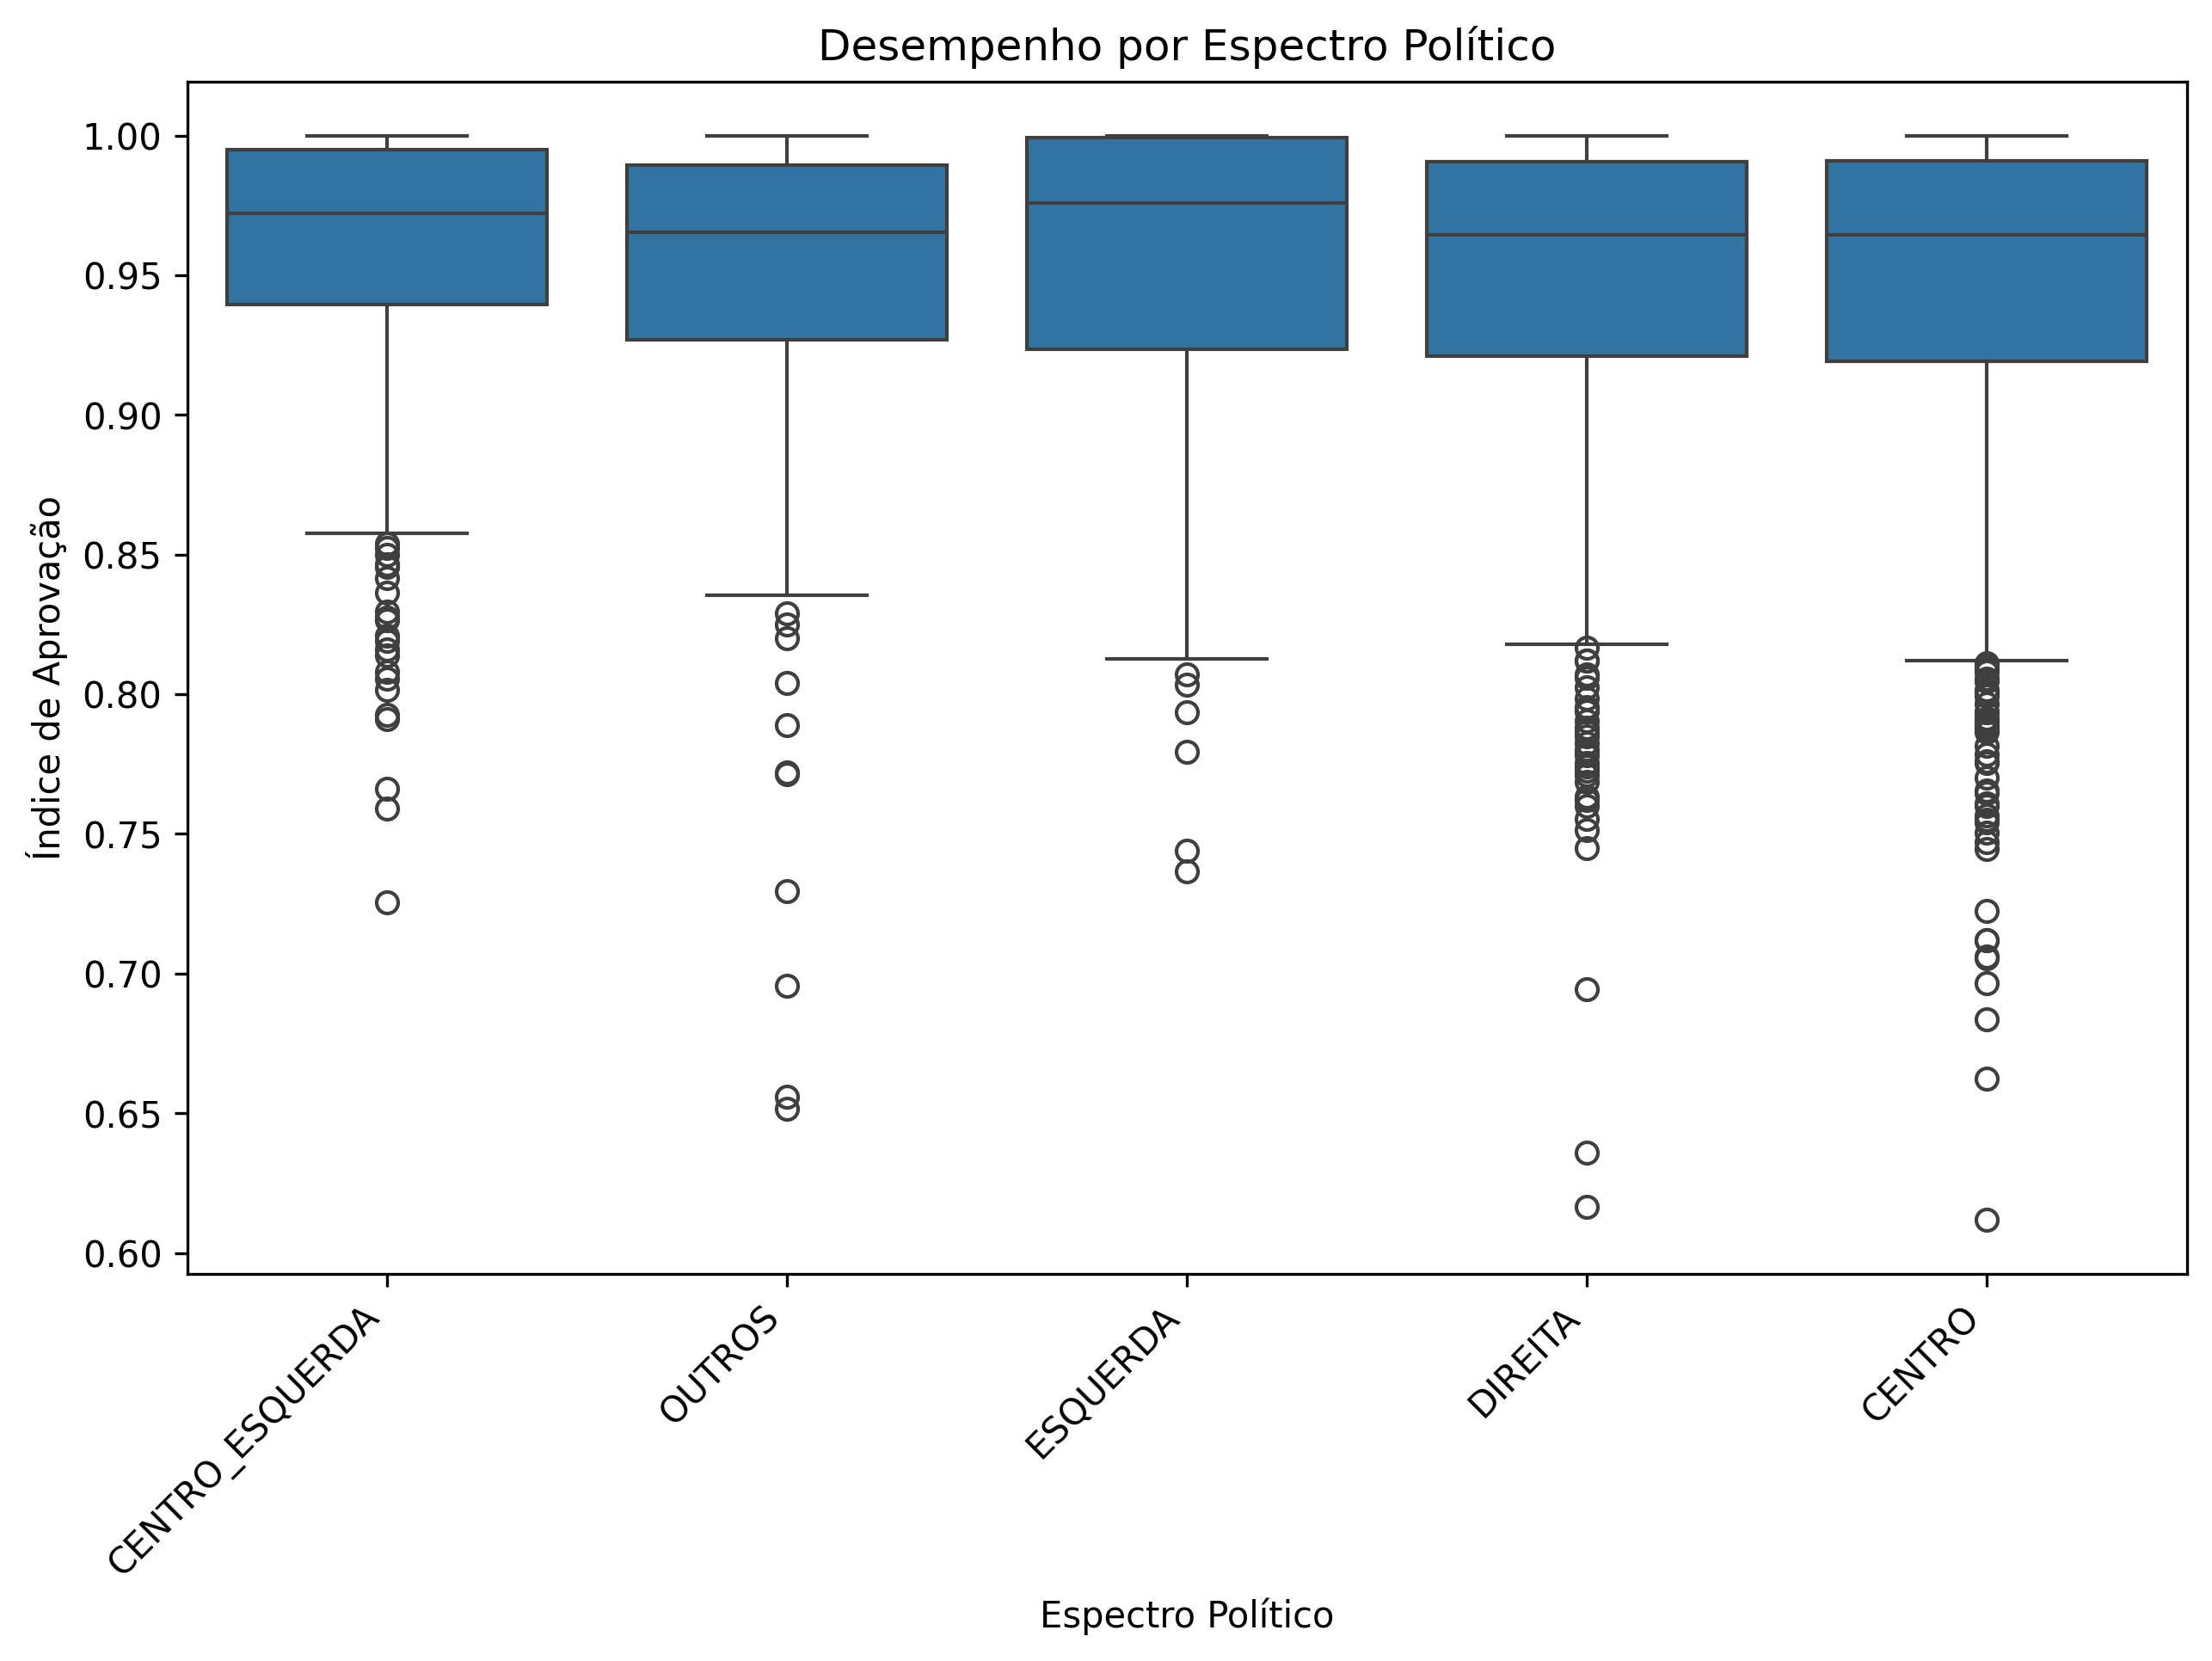
\includegraphics[width=\textwidth]{assets/desempenho_espectro.png}
            \tiny Observamos diferenças nas medianas e distribuições do índice de aprovação entre os espectros.
        \end{column}
        \begin{column}{0.5\textwidth}
            \textbf{Distribuição Geral}
            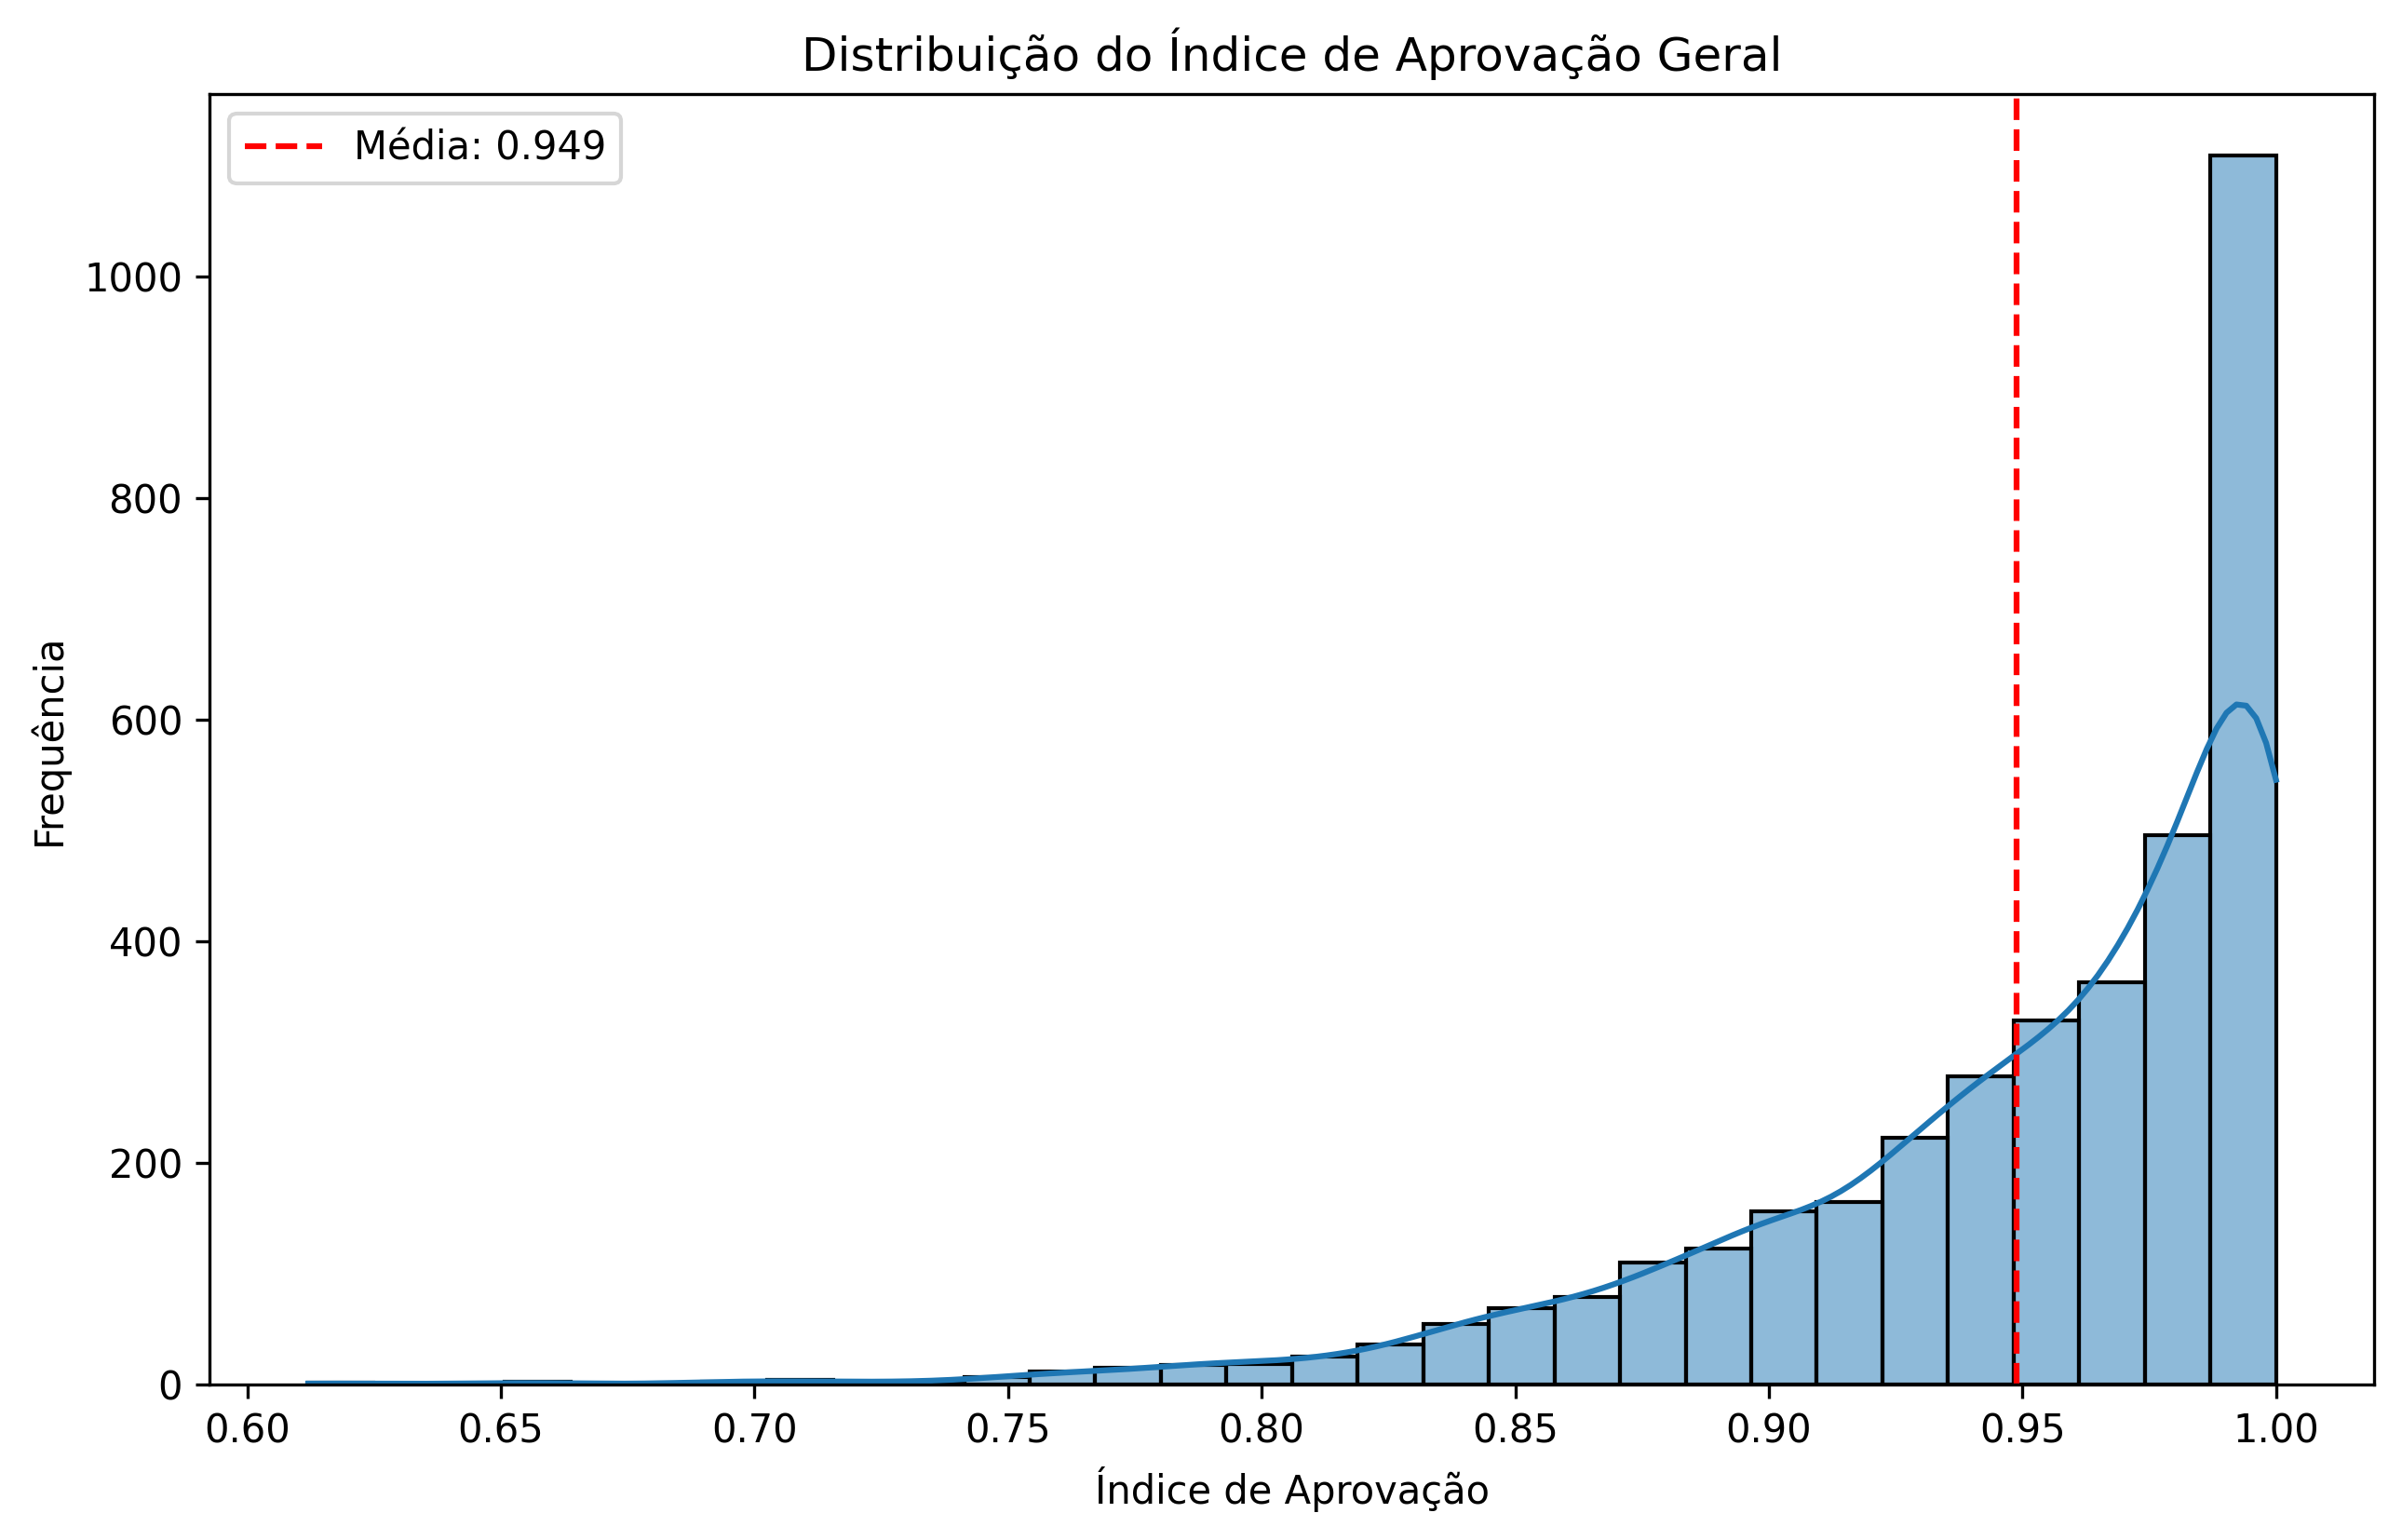
\includegraphics[width=\textwidth]{assets/distribuicao_indice.png}
            \tiny A maioria dos municípios se concentra em uma faixa de alta aprovação, indicando desbalanceamento de classes.
        \end{column}
    \end{columns}
\end{frame}

% --- Slide 4: Modeling Results ---
\begin{frame}{Resultados da Modelagem Preditiva}
    \textbf{Objetivo:} Prever se a performance será "Alta" ou "Baixa".\\
    \textbf{Modelo Campeão:} RandomForest (ROC AUC $\approx$ 0.80)
    \vfill
    \begin{figure}
        \centering
        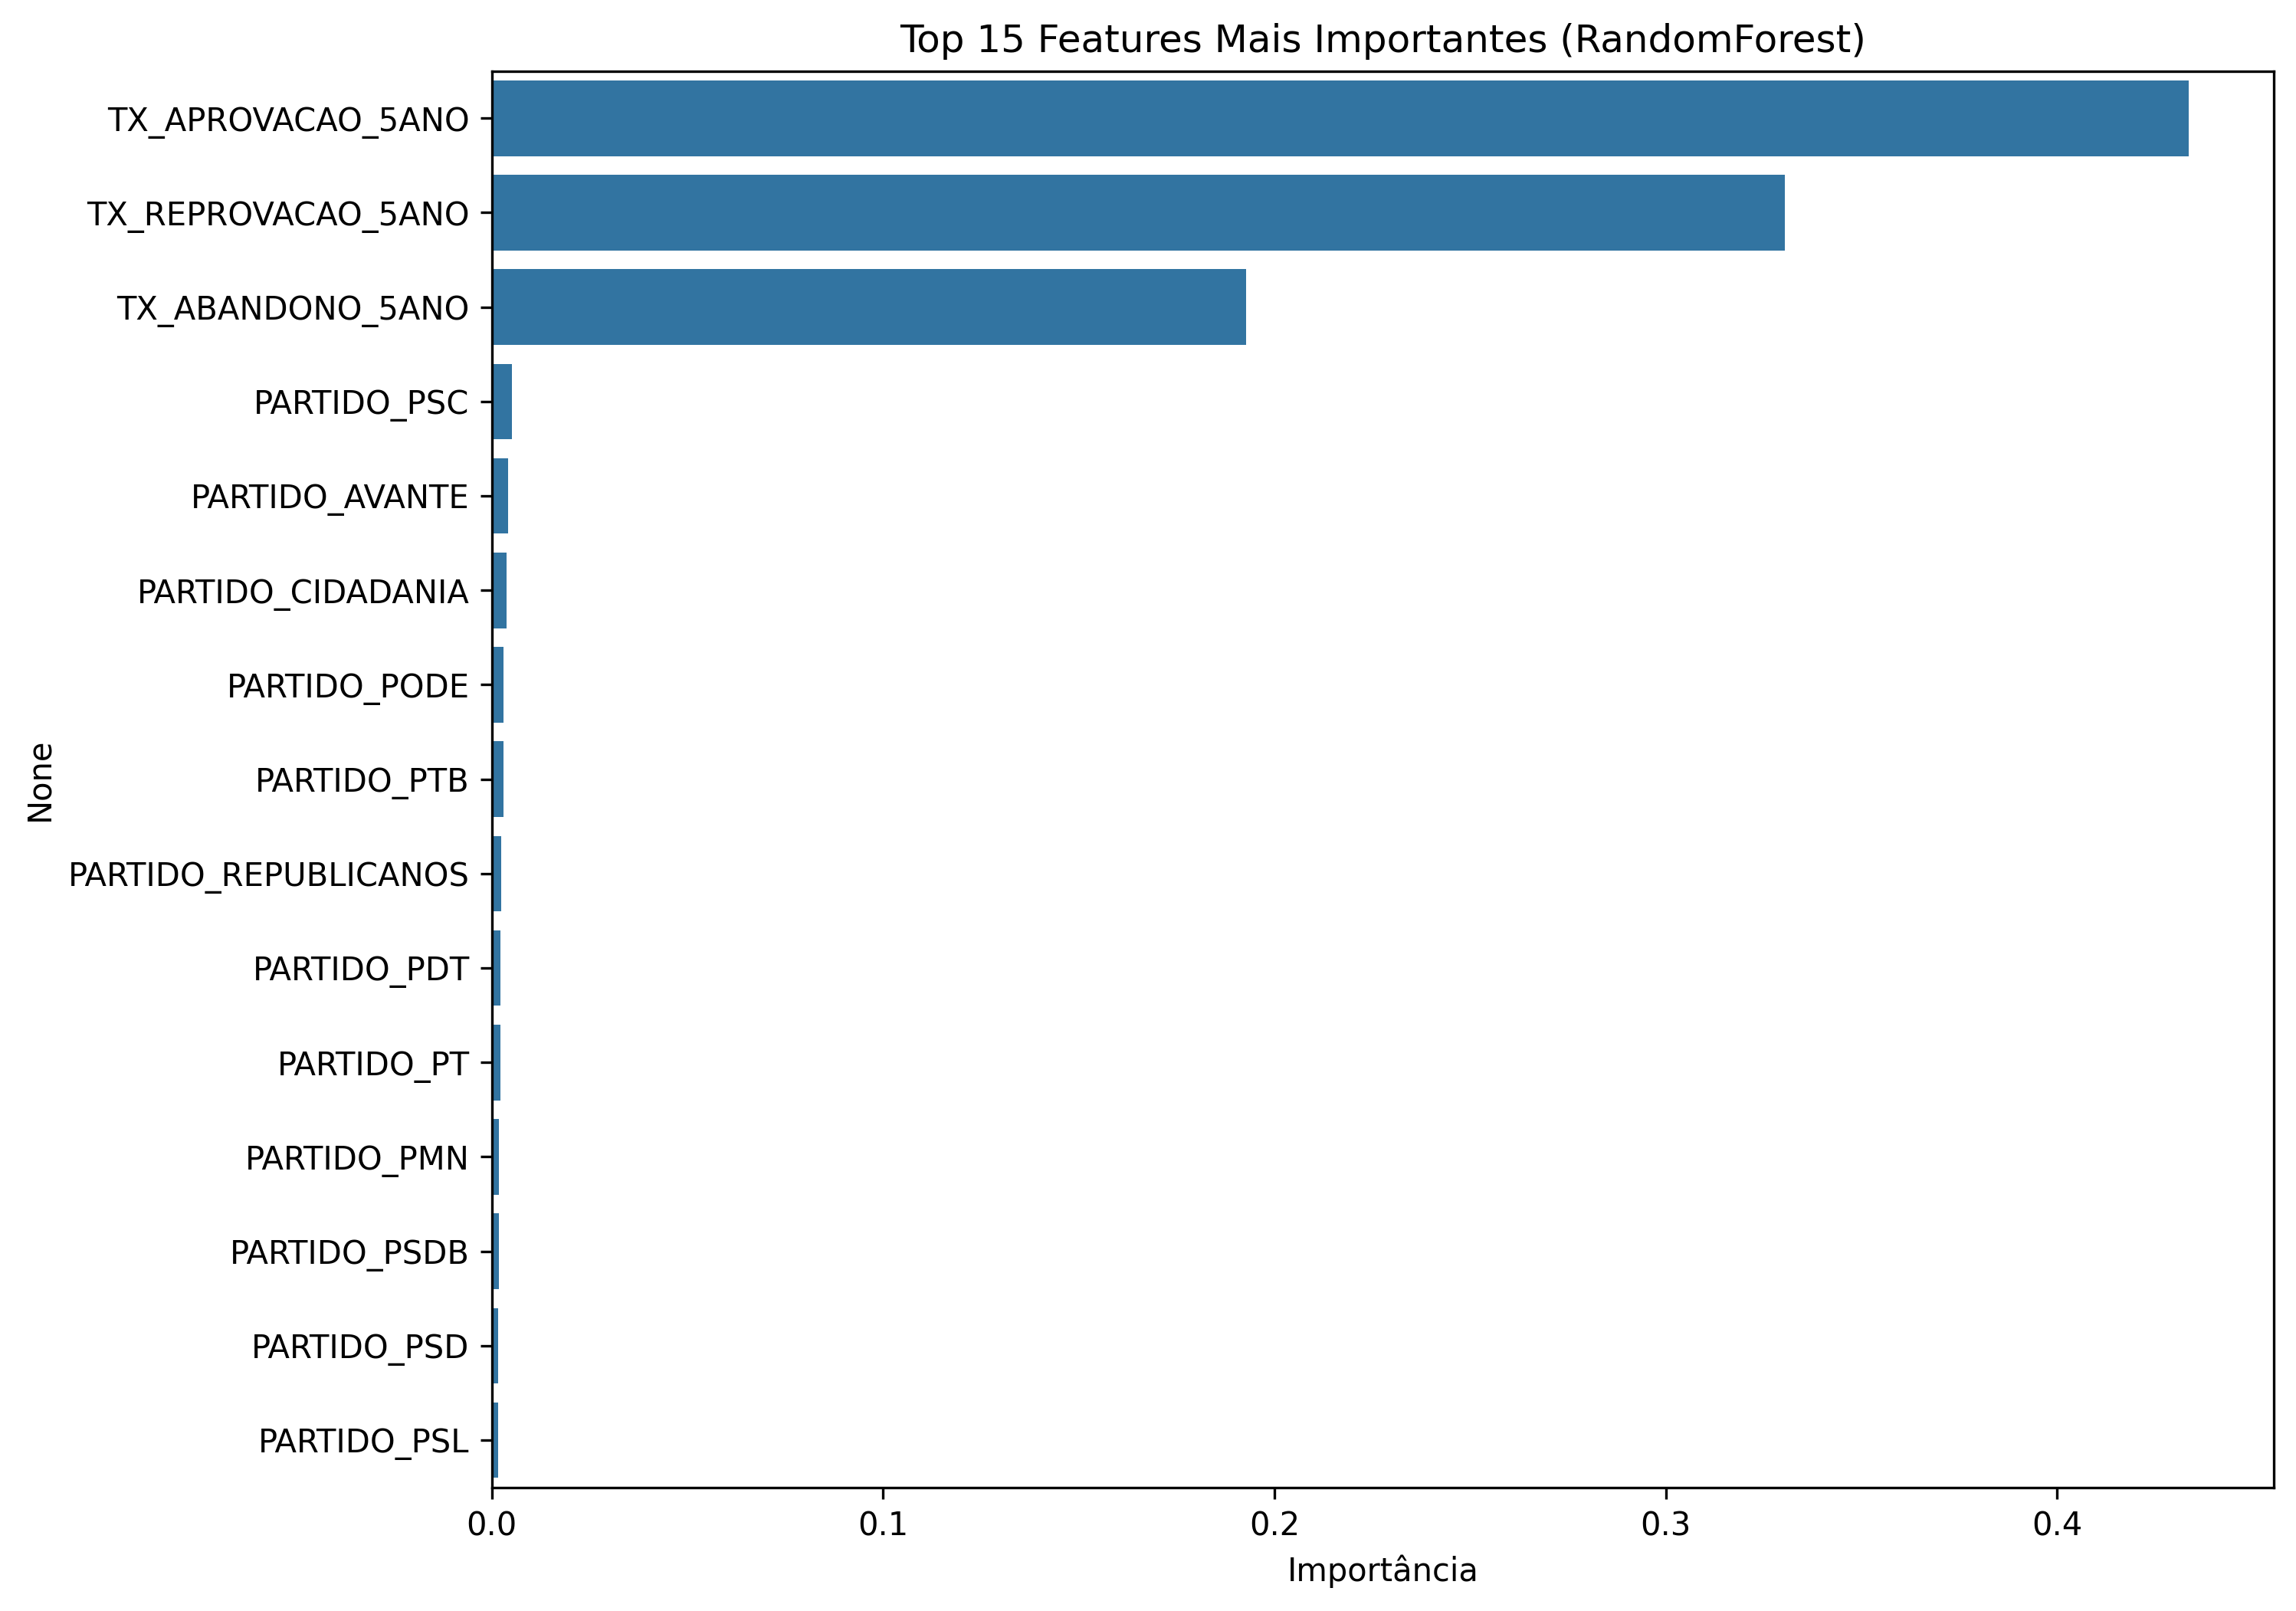
\includegraphics[width=0.8\textwidth]{assets/feature_importance.png}
        \caption{As taxas de aprovação do 5º ano são o fator mais preditivo, seguidas por fatores partidários específicos.}
    \end{figure}
\end{frame}

% --- Slide 5: API Demonstration ---
\begin{frame}[fragile]{Demonstração da API}
    \textbf{Endpoint:} \texttt{POST /predict}
    \vfill
    \textbf{Exemplo de Requisição (`curl`):}
    \begin{semiverbatim}
    curl -X POST http://127.0.0.1:5000/predict \\
    -H "Content-Type: application/json" \\
    -d '{
        "PARTIDO": "PSDB",
        "TX_APROVACAO_5ANO": 0.85,
        ...
    }'
    \end{semiverbatim}
    \vfill
    \textbf{Resposta da API:}
    \begin{semiverbatim}
    {
      "performance_label": "Alta",
      "prediction": 1,
      "probability": { "alta": 0.67, "baixa": 0.33 }
    }
    \end{semiverbatim}
\end{frame}

% --- Slide 6: Conclusion ---
\begin{frame}{Conclusão e Próximos Passos}
    \begin{block}{Conclusões}
        \begin{itemize}
            \item Pipeline MLOps completo e automatizado foi construído com sucesso.
            \item Desempenho educacional anterior é o preditor mais forte.
            \item Afiliação partidária demonstrou ser um fator preditivo secundário.
        \end{itemize}
    \end{block}
    \vfill
    \begin{block}{Próximos Passos}
        \begin{itemize}
            \item Enriquecer o dataset com variáveis socioeconômicas (IDH, PIB).
            \item Experimentar com modelos de Gradient Boosting (XGBoost).
            \item Implementar o deploy contínuo (CD) da API.
        \end{itemize}
    \end{block}
\end{frame}

% --- Final Slide ---
\begin{frame}
    \begin{center}
        \Huge{\textbf{Obrigado!}}
        \vfill
        \Large{Perguntas?}
    \end{center}
\end{frame}

\end{document}
